%!TEX root=../slr.tex
\section{Conduction}
\label{sec:conduction}
\subsection{Search Results}
\label{sub:the_search}

The search phrase, as was determined in Section~\ref{sec:methods} was
run through the selected libraries using a specialised software called
\emph{Publish or Perish}~\cite{Harzing}. This software allows exporting
search results into a comma-separated-values (csv) file, that is easily
imported into a spreadsheet program such as Microsoft Excel and making
the process a lot more expedient. Since one of the electronic search
engines that were used was Google Scholar, which is much more powerful
and broad than the other libraries, it demanded some special attention
due to the many repeated entries that we were sure to find using this
method. The flowchart depicted in Figure~\ref{fig:flowchart} illustrates
the search stages. In the end, our search resulted in a total of 61
articles in all libraries. Almost half of them (29 in 61) were excluded
due to the application of some exclusion criteria. The high number of
excluded papers is mostly a result of Google Scholar's search broadness
(25 excluded results vs 3 in Scopus and 1 in WoS). 19 of the entries
retrieved using Scopus and WoS were already in GS, which combined with
the numerous exclusions, resulted in a final number of 13 papers. A
summary of these results can be found in Table~\ref{tab:search_results},
and the list of selected papers can be seen in
Table~\ref{tab:selected_papers}.

\begin{figure}[htpb]
    \centering
    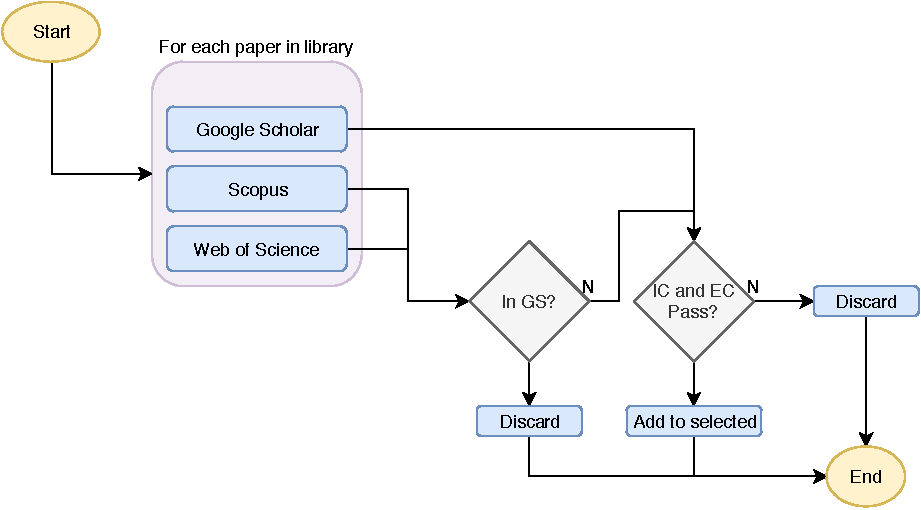
\includegraphics[width=\linewidth]{img/pdf/asd_flowchart.pdf}
    \caption{Conduction stage flowchart. Libraries are searched
    independently through \emph{Publish or Perish}, but results must be
    checked to ensure they are not counted twice, due to the imbalance of
    power between GS's search engine and the others.}
    \label{fig:flowchart}
\end{figure}

\begin{table}[htb]
\centering
\caption{Search results summary.}
\label{tab:search_results}
\begin{tabular}{@{}lccccr@{}}
\toprule
\textbf{Library} & \textbf{Results} & \textbf{Excluded} & \textbf{In GS} & \textbf{Final} & \textbf{Weight in study} \\ \midrule
\textbf{GS} & 37 & 25 & 0 & 12 & 92,31\% \\
\textbf{Scopus} & 15 & 3 & 12 & 0 & 0\% \\
\textbf{WoS} & 9 & 1 & 7 & 1 & 7,69\% \\
\midrule
\textbf{Total}& \textbf{61} & \textbf{29} & \textbf{19} &\textbf{13} & \textbf{100,00\%} \\ \bottomrule
\end{tabular}
\end{table}

\begin{table}[htb]
    \centering
    \small
    \caption{References and relevant data for the selected papers,
        including their score, which was calculated according to
        Equation~\ref{eq:score}.}
    \label{tab:selected_papers}
    \begin{tabular}{@{}llllll@{}}
    \toprule
    \textbf{Number} & \textbf{Reference} & \textbf{Quartile} &
    \textbf{Citations} & \textbf{Year} & \textbf{Score} \\ \midrule
    \textbf{1} & \cite{Hartl2006} & 1 & 35 & 2006 & 2,69 \\
    \midrule
    \textbf{2} & \cite{Hartl2005} & 1 & 2 & 2005 & 0,14 \\
    \midrule
    \textbf{3} & \cite{Laepple2004} & 1 & 30 & 2004 & 2,00 \\
    \midrule
    \textbf{4} & \cite{Pundt2005} & 2 & 1 & 2005 & 0,05 \\
    \midrule
    \textbf{5} & \cite{Murphy2003} & 3 & 6 & 2003 & 0,19 \\
    \midrule
    \textbf{6} & \cite{Frins2006} & 1 & 8 & 2006 & 0,62 \\
    \midrule
    \textbf{7} & \cite{Johansson2009} & 2 & 26 & 2009 & 1,95 \\
    \midrule
    \textbf{8} & \cite{ODriscoll2003} & 4 & 0 & 2003 & 0,00 \\
    \midrule
    \textbf{9} & \cite{Pundt2006} & 1 & 12 & 2006 & 0,92 \\
    \midrule
    \textbf{10} & \cite{Pundt2005b} & 1 & 42 & 2005 & 3,00 \\
    \midrule
    \textbf{11} & \cite{ODriscoll2003a} & 4 & 1 & 2003 & 0,02 \\
    \midrule
    \textbf{12} & \cite{Mettendorf2006} & 1 & 4 & 2006 & 0,31 \\
    \midrule
    \textbf{13} & \cite{Casaballe2017} & 1 & 2 & 2017 & 1,00 \\ \bottomrule
    \end{tabular}
\end{table}

\subsection{Discussion}
\label{sub:discussion}

The final goal of this study was to identify a possible means of
approaching DOAS tomography in an innovative way. For this, we have used
the information contained in the 13 selected articles, trying to find
some commonalities and patterns that can be useful to us.

One of the first patterns that can be observed is that most of the
literature in this subject was written on the application of active DOAS
systems, i.e., systems that use some kind of artificial light source to
perform their spectroscopic analysis. Active systems are instrumentally
much more complex than passive systems. However, they allow a more
thorough analysis of the studied trace gases. In addition, passive
systems also imply dealing with much more complicated physical
phenomena, such as radiative transfer equations. Another almost
immediate observation that can be raised is that many studies (6/13)
originate from the BABII campaign, which was an initiative of the
Institute for Meteorology and Climate Research in Karlsruhe, Germany.
The campaign intended to experimentally monitor the traffic emissions in
the A656 motorway~\cite{Laepple2004}. Judging by the number of papers
this initiative created, this was the largest tomographic DOAS campaign
ever made.

All of the active DOAS solutions that were selected in our study are
Long Path DOAS applications. Also all of the systems were custom built for
their particular study or campaign. The group associated with the BABII
campaign had two telescopes with diameters in the order of 200 mm and a
focal length of around 1 m to simultaneously emit the light from a Xenon
lamp towards a constellation of 8 retro-reflectors, which were assembled
on two towers, on both sides of the motorway that connects Heidelberg
with Mannheim~\cite{Pundt2005}. The same assembly and instruments were
used by the other papers of the group, namely~\cite{Hartl2006, Poehler,
Laepple2004}. The paper identified in ~\cite{Mettendorf2006} is also
from the same group, but the article had a very different approach and
purpose. Instead of aiming to map a given region (which in this case
would be a motorway vicinity), the authors wanted to validate the
two-dimensional reconstruction technique that would be used in the other
studies, by conducting an indoor experiment using three multibeam
instruments consisting in a telescope (1.5 m  focal length and 300 mm
diameter) that acted as both emitter and receiver, together with three
fixed "towers" that held the retro-reflectors and a Xenon lamp as light
source.

The work done by the group that wrote~\cite{Stutz2016} took a different
but similar approach to a completely different application. They used an
LED light source with a narrow wavelength interval light in the UV
region (around 290 nm) and a custom built instrument assembly that was
used as a fence line monitor for a refinery in Los Angeles and then to
monitor the two-dimensional concentration fields for Benzene, Toluene
and Xylenes in Houston, Texas. Both experiments have found the system's
findings to be satisfactory, and the device was able to map the
concentration for the target chemical species with success. In addition
to this study's inherent research interest, it is also good to note that
Stutz' paper describes a system that could easily be converted to a
commercial product.

The research group at the Cork Institute of Technology, in Ireland, has
approached the problem in a different way. In the three papers from this
group~\cite{Murphy2003, ODriscoll2003, ODriscoll2003a} that were
selected for this study, the authors present and discuss three new
tomographic approaches. The first is a new optical design, based on a
multipath assembly that allows for a significant increase in the number
of optical paths produced by a single light source; the second was an
attempt at reconstructing the tomographic image through the use of
evolutionary algorithms; and the third was the application of the
tomographic DOAS technique to a simulated urban canyon. These three
articles were deemed relevant for this study because they do have
technological novelty. However, it should be noted that on a more
literary level, the three papers were among the weakest in the selected
group, and were only published as conference proceedings.


%%%%%%%%%%%%%%%%%%%%%%%%%%%%%%%%%%%%%%%%%%%%%%%%%%%%%%%%%
%       Editing on Asus Compta
%%%%%%%%%%%%%%%%%%%%%%%%%%%%%%%%%%%%%%%%%%%%%%%%%%%%%%%%%
Regarding passive DOAS applications, the two papers we have found come
with two completely different paradigms. The first
article~\cite{Johansson2009} was written in 2009 and details the
application of a tomographic inversion algorithm to a scanning DOAS
application, designed to work with trace gas plumes like the ones above
volcanoes or power stations. The team present a system composed of two
DOAS devices, with sufficient distance with themselves as to allow
tomographic reconstruction, but sufficiently small to allow the light
path to be considered a straight line from the point of last scattering
to the detector. The authors applied an adapted version of the Lower
Third Derivative (LTD) algorithm to the projections obtained by pointing
the set of fixed DOAS apparatus towards the plume in different angles.
Besides simulations for their proposed method, the authors have also
conducted practical experiments, both over a power plant in Spain and a
volcano in Italy. Results from these experiments display a good
agreement between reality and simulation results, proving the
technique's validity.

The second Passive DOAS application is a paper published by Frins et
al.~\cite{Frins2006}. In this study, the researchers detail a particular
application in which they measure light coming from bright and
nonreflecting sun-illuminated objects in their field of view. They use
this light to retrieve column density values for a number of trace
gases. The proposed method also includes a way with which to remove the
stratospheric contribution that appears in the measured light besides
the target column. The authors discuss how radiative transfer can
influence measurements, but they also present a number of approaches to
mitigate this problem, ensuring the validity of their approach.  Besides
presenting the method, the authors also describe an experiment they
conducted by assembling and manoeuvring a DOAS system on top of a
building in Heidelberg, Germany.
 
% \subsubsection{Instrument}
% \label{ssub:instrument}

% Instrumentation description is present in 7 of the 8
% (\cite{Hartl2006,Laepple2004,
% Mettendorf2006,Olaguer2017,Poehler,Pundt2005, Stutz2016}) selected
% articles. Stutz2016~\cite{Stutz2016}, Pundt2005~\cite{Pundt2005} and
% Mettendorf2006~\cite{Mettendorf2006} present the highest level of
% detail.

% In Stutz2016~\cite{Stutz2016}, the authors used a newly developed Long
% Path DOAS instrument for the study of atmospheric concentration of
% Benzene, Toluenes and Xylenes. This instrument's main innovation is its
% light source, which consists in a double LED (255nm and 265nm) assembly.
% This system's telescope is a homebuilt telescope with a focal length of
% 120 cm and a 12 inch diameter aluminum coated main mirror, mounted on a
% high accuracy motorised pan and tilt unit from Newark Systems. The
% telescope is used both as emitter and receiver, therefore the system
% needs a reflector. Stutz used a quartz corner cube reflector array,
% with an individual reflector diameter of 57 mm and the number of
% reflector ranging from 10 to 25 (depending on the path length). For
% detection, the system relied on a UV-enhanced PIXIS 256 CCD detector
% from Princeton Instruments on an Acton spectrometer with 300 grating and
% $\approx$0,3 nm spectral resolution, which was stabilised to -35ºC.

% Pundt2005~\cite{Pundt2005} was conducted during the BAB II motorway
% campaign. The team was working with the goal of performing a tomographic
% measurement of vehicle polution along a certain motorway between
% Heidelberg and Mannheim. For that, they used an assembly of two
% telescopes and eight reflectors, rendering a total of 16 light paths,
% then used to perform a tomographic reconstruction of the trace gas
% detection in that region. The telescopes used had a focal length of 150
% and 80 cm, with respective diameters of 300 and 200 mm. Both assemblies
% used Acton spectrometers. One used the Acton 500, with 0,5 nm spectral
% resolution in the range between 295 and 375 nm; the other used an Acton
% 300, with 0,4 nm spectral resolution between 295 and 355 nm. In both
% cases, the sensor used was a 1024 pixe Photo Diode Array (PDA),
% thermally stabilised at -15ºC. The telescopes were pointed towards two
% towers which beared the reflectors, set at heights of 10, 20, 30 and 40
% m from the ground. The system's geometry and distances are shown in
% Figure~\ref{fig:babii_geometry}.

% \begin{figure}[htb]
%     \centering
%     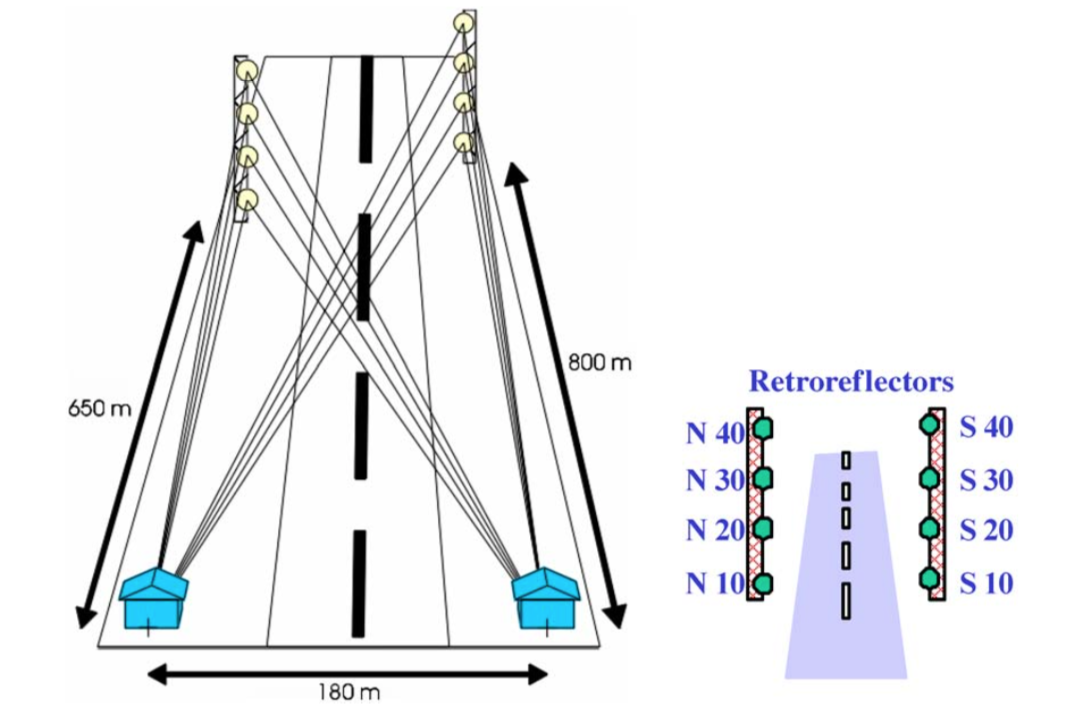
\includegraphics[width=0.8\linewidth]{img/babii_geometry.png}
%     \caption{Schematic representation of the BABII campaign
%     experiment~\cite{Pundt2005}.}\label{fig:babii_geometry}
% \end{figure}

% In Mettendorf2006~\cite{Mettendorf2006}, the authors validated
% two-dimensional LP-DOAS tomography through an indoor experiment. To this
% end, they have used three multibeam instruments, which consisted in a
% telescope with a focal length of 1,5 m and 300 mm in diameter, which was
% also used as emitter and receiver. The system used a broad spectrum
% Xenon lamp as light source, though no details are given. The experiment
% assembly included the careful positioning of plane mirrors and 6 cm
% diameter corner cube reflectors, used to create a total of 39 light
% paths (13 for each multibeam instrument). Telescope, mirror and
% reflector positions are illustrated in Figure~\ref{fig:mettendorf_geom}.

% \begin{figure}[htb]
%     \centering
%     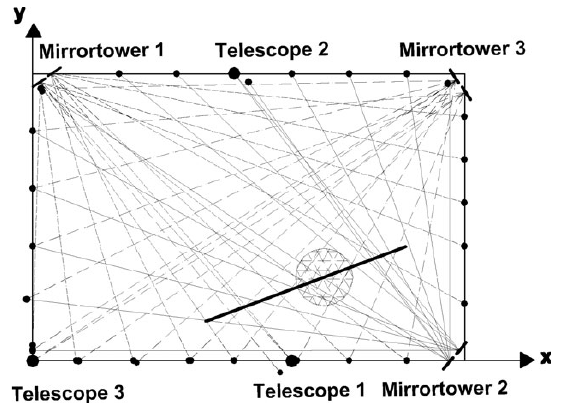
\includegraphics[width=0.8\linewidth]{img/mettendorf.png}
%     \caption{Mettendorf2006~\cite{Mettendorf2006} experiment geometry,
%     detailing position of telescopes (large filled dots), mirrors (small
% lines in upper corners), reflectors (small dots along edges), test
% samples (hatched circle), light paths (thin lines) and the movement path
% for the sample (thick diagonal line).}\label{fig:mettendorf_geom}
% \end{figure}

% As for the other 4 less detailed instrument description, three
% (Hartl2006~\cite{Hartl2006}, Poehler~\cite{Poehler} and
% Laepple2004~\cite{Laepple2004}) are from the same group as
% Pundt2005~\cite{Pundt2005} and Mettendorf2006~\cite{Mettendorf2006}, and
% therefore use the same or similar hardware.
% Olaguer2017~\cite{Olaguer2017}, on the other hand, is the companion
% paper of Stutz2016~\cite{Stutz2016}, and therefore gives a description
% of the same instrumentation, though in a less detailed manner.

% \subsubsection{Algorithm}
% \label{ssub:algorithm}

% The reconstruction algorithm is the most important part of our study, as
% we already demonstrated by the weight it is given in our quality
% evaluation model (see Subsection~\ref{sub:quality_assessment}).
% Algorithm descriptions are present in 6 of the 8 selected
% articles:~\cite{Hartl2006, Laepple2004, Mettendorf2006, ODriscoll2003,
% Olaguer2017, Pundt2005}. The most complete descriptions are featured in
% Hartl2006~\cite{Hartl2006}, Laepple2004~\cite{Laepple2004} and
% ODriscoll2003~\cite{ODriscoll2003}.
% Mettendorf2006~\cite{Mettendorf2006}, Olaguer2017~\cite{Olaguer2017} and
% Pundt2005~\cite{Pundt2005} approach the reconstruction algorithms with
% less emphasis or in a less detailed way.

% In Hartl2006~\cite{Hartl2006}, the research team describe their
% discretisation process, reconstruction methods, grid translation methods
% and error estimation and quality assessment, with the greatest level of
% detail being given to the latter.

% The paper also focuses in the comparison SIRT and ART results for the
% test samples, which consisted in up to four Gaussian concentration
% profiles, which were randomly arranged in a 100x100 (a.u.) test field,
% in six different geometries and  with up to 36 known light paths.

% Furthermore, Hartl2006~\cite{Hartl2006} discusses how the choice of the
% reconstruction grid affects both the reconstruction error and
% reconstruction area integrals, the possibility of the existence of
% background concentration influencing equation constraints and
% reconstruction results, and how the whole system would behave were its
% geometry any different, namely regarding light paths and number of
% telescopes. 

% The next algorithm-oriented paper is Laepple2004~\cite{Laepple2004}. In
% this article, the group discussed several discretisation approaches,
% their drawbacks and advantages. Still on discretisation, they approach
% the problem of resolution, and the necessary balance between physical
% accuracy and the need for \emph{a priori} information which arises from
% increasing it. Afterwards, the group presents some strategies for
% solving the linear system that results from discretising the
% concentration field and how to take error into account.

% For their reconstructions, the group chose to adapt ART, SIRT, and SART
% . These adaptations were described and detailed in the article's third
% section, before the error estimation procedures adopted in their case.
% Finally, the team presents how they chose to optimise reconstruction in
% several aspects, including the generation of test plumes and
% optimisation for the BABII campaign, which was the parent project of
% this article. 

% ODriscoll2003~\cite{ODriscoll2003} also covers the algorithm
% extensively. While this paper is considerably shorter that the previous
% two, it provides a detailed (on an iteration basis) description for ART
% and SIRT. In addition, and perhaps of greater interest, the paper's
% authors suggest a different approach to solving the reconstruction
% matrix, different from the algebric methods already presented: an
% evolutionary algorithm.

% An evolutionary algorithm is a mathematical method of solving complex
% problems, which mimics or is in any form based on the process of natural
% selection. These algorithms have, according to the paper's authors and
% their references, been shown to be extraordinarily powerful.

% The research team have applied a Differential Evolution algorithm to the
% reconstruction process and provide a detailed description of how they
% have done this.

% The other two articles which mention the algorithm are
% Mettendorf2006~\cite{Mettendorf2006} and Pundt2005~\cite{Pundt2005}.
% Both these studies were conducted under the same project as
% Laepple2004~\cite{Laepple2004} and Hartl2006~\cite{Hartl2006} and
% therefore their algorithm descriptions and methods draw heavily on
% these two studies.


% \subsubsection{Software}
% \label{ssub:software}

% Of the 8 selected articles, only 3 mention the software used. Even these,
% do not go into any detail of the reasons that led to that specific
% usage. 

% In Mettendorf2006~\cite{Mettendorf2006}, the team used TOMOLAB
% for the calculation of the modelled column densities of their
% experiment. In Pundt2005~\cite{Pundt2005}, spectral analysis was
% performed using the \emph{MFC Software}. Finally,
% Stutz2016~\cite{Stutz2016} used the DOASIS software for control and
% automation purposes, and does not explicitly mention its use for
% spectral analysis purposes, although this is likely.

% \subsubsection{General Observations}
% \label{ssub:general_observations}

% While this is not a part of the discussion \emph{per se}, we believe it
% makes sense to make some general observations about the data which wwe
% had to analyse.

% The first important mention is the BABII campaign. This study, which ran
% in 2001 and aimed to quantify polution from the A656 motorway between
% Heidelberg and Mannheim produced a significant part of the literature
% which we analysed.

% Another point which should be addressed is that all DOAS tomography
% efforts detected in this search were based on active DOAS technology.
% This only means that the DOAS systems all employed an artificial light
% as a light source.

% A final remark is due to the prevalence of algebric methods for
% solving the discretisation and reconstruction problem, namely ART, SART
% and SIRT. 

\subsection{Validity Threats}
\label{sub:validity_threats}

When writing an MS or an SLR, authors always have to analyse their
findings and methods in order to mitigate potential sources of error or
lack of validity. This is called a validity threat analysis.

There are two main families of validity threats. They can be internal,
i.e., they come from the methods employed used in conducting the study;
or external, which means that the threat comes from the applicability
(or lack thereof) of the effects observed in the study, outside of its
scope.

On the level of internal validity of our study, two main observations
come to mind:
\begin{description}
    
    \item[Relevant papers left out] The very low number of found studies
        could be an indication that our inclusion and exclusion filters
        were set in a too restrictive manner. It could also happen that
        some relevant papers were not found due to being written in such
        a way that the libraries' search engines did not find them with
        our search phrase. This same problem would also occur if for
        some reason, an important library was left out of the study, and
        therefore not searched. We mitigate all these risks by selecting
        a purposefully broad search phrase, by using powerful general
        search engines (eg.  Google Scholar) and by running several
        undocumented test-runs with other search phrases. A common
        strategy used for tackling this kind of threat is to extend the
        study through snowballing, which in our case would not make a
        great difference, due to the fact that many of the identified
        papers reference one-another.
    
    \item[Quality of selected papers] Papers were selected according to
        the inclusion criteria defined in Section~\ref{sec:methods}.  In
        the same section, we have discussed how the articles were
        assessed regarding their quality, and stated that the method
        with which the articles are ranked in this regard exclusively
        depends on the number of citations. This number, in a field with
        so few papers in the literature, will always be small and can be
        deceiving if one tries to read the paper's relevance with this
        score. 

\end{description}

On the external threat plane, we contend with the applicability of our
findings outside our study. The study itself had the clear purpose of
identifying a \emph{vector of approach} for an innovative product in
DOAS tomography. As long as we accomplish this objective, we can regard
it as externally valid, even if it is of little use outside the field of
study.

